% !TEX root = mythesis.tex

%==============================================================================
\chapter{Conclusion and Outlook}
\label{sec:conc}
%==============================================================================
\begin{figure}[h!]
\centering
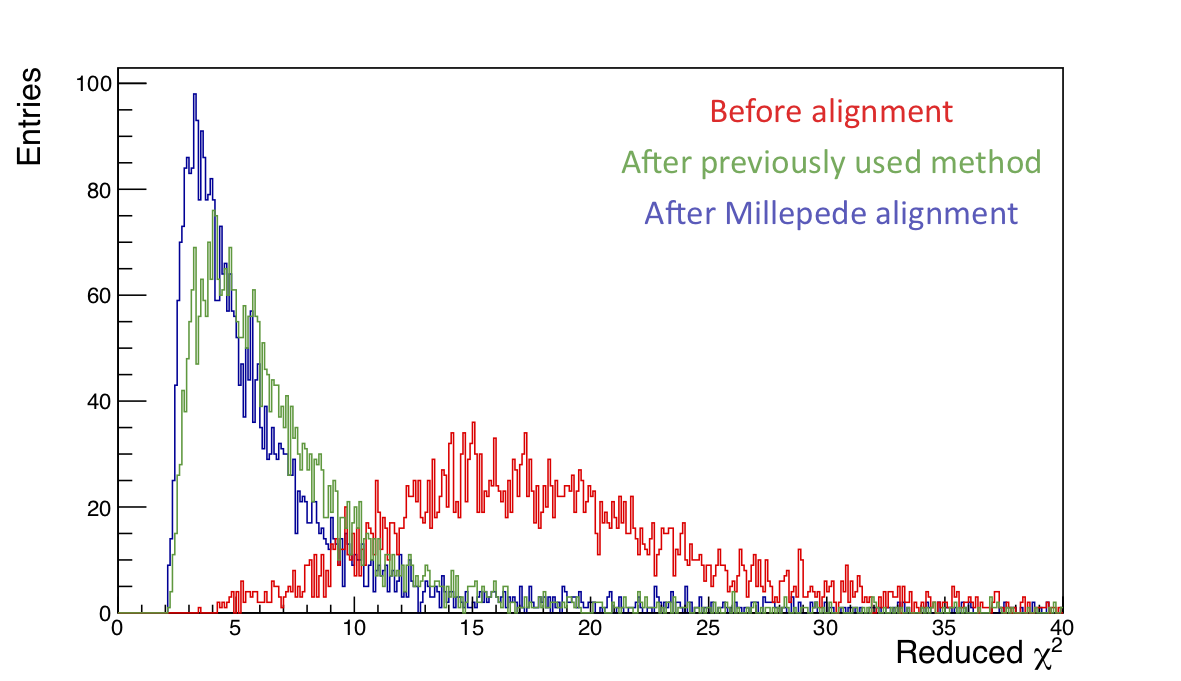
\includegraphics[width=0.85\textwidth]{thesis_figures/chi2_comp_conclusion_2.png}
\caption{$\chi^2_{red}$ distribution for selected tracks showing the impact of Millepede alignment.}
\label{fig:red_chi2_4}
\end{figure}

\section*{Alignment}
During the course of this thesis a successful positional and angular alignment was performed for run 3211 using the Millepede alignment tool. As it is evident from fig.(\ref{fig:red_chi2_4}), a \textbf{run by run alignment} is required for the NA64 experiment to maximize the positional resolution of the tracking detectors. This in turn will make the beam momentum determination more precise which is a high priority for NA64. \textbf{Millepede} is one of the best available tools, is now compatible with the NA64 setup and can be used for this purpose.

\subsection*{Outlook}
Since the results from the alignment also depend on the individual detector resolution a better estimate of the resolutions for both Micromegas and GEMs might be required before a final run by run alignment is performed.

Another global parameter which can be looked into is the forward or backward tilt of the detector. If the detector is tilted in either one of these directions it can lead to a missallocation of hits, in turn affecting track fitting since CORAL assumes the detector to be perfectly aligned. This misallocation can be fixed by varying the pitch of the detector which is the distance between the readout strips. Even though the pitch of the detector is fixed by construction, the movement simply mimics the tilt of the detector and is generally of the order of few $\mu m$. Although the expected impact is very small it is something which can be looked into more since it is already operational in Millepede. A future z positional alignment is also available and can also be looked into in the future.

\section*{MC Reconstruction}
The second task which was performed during this thesis is the reconstruction of the MC simulation for the 2018 setup in CORAL. This involved transforming the output of the simulation which is obtained from the collaboration to a format which is compatible with CORAL. The reconstruction is confirmed to be working. As a proof of principle the reconstructed beam momentum distribution is checked and confirmed to be reasonable. An attempt was also made to check the $A'$ reconstruction by looking at the angular distribution of its decay products. The distribution was as expected for the simulated $A'$ mass $m_{A'}$. The MC simulation is also described briefly in the thesis.

\subsection*{Outlook}
The angular dependence of the fitted beam momentum needs to be looked into further. This might add to the uncertainties during the determination of the reconstructed beam momentum. It seems to be related to the track fitting algorithm used by CORAL. Further rare dimuon events, $e^-Z\rightarrow e^-Z\gamma;\gamma\rightarrow \mu^{+} \mu^{-} $ can be used to estimate the efficiency of the MC reconstruction in CORAL. Such events could not be observed during this thesis since the current MC sample which was reconstructed is too small. Bigger samples of simulation already exist and can be processed in the future. Even though the reconstruction was done for the visible mode setup, it is also functional for the invisible mode since all of the detectors implemented are the same except for the WCAL. Hence, MC reconstruction for the invisible mode can be easily done by just plugging in the setup specific detectors table. The results of this thesis help further the goal of performing a full physics $A'$ analysis in CORAL in the future.


%%% Local Variables:
%%% mode: latex
%%% TeX-master: "mythesis"
%%% End:
